\documentclass{jarticle}
\usepackage[dvipdfmx]{graphicx}
\title{オブジェクト指向最終レポート}
\author{学生番号:2014SE042 氏名:加納 辰真}

\begin{document}
\maketitle

\newpage

\section{問題3の実行結果}
図 \ref{emb} が問題3の実行結果です.

\begin{figure}[ht]
  \begin{center}
    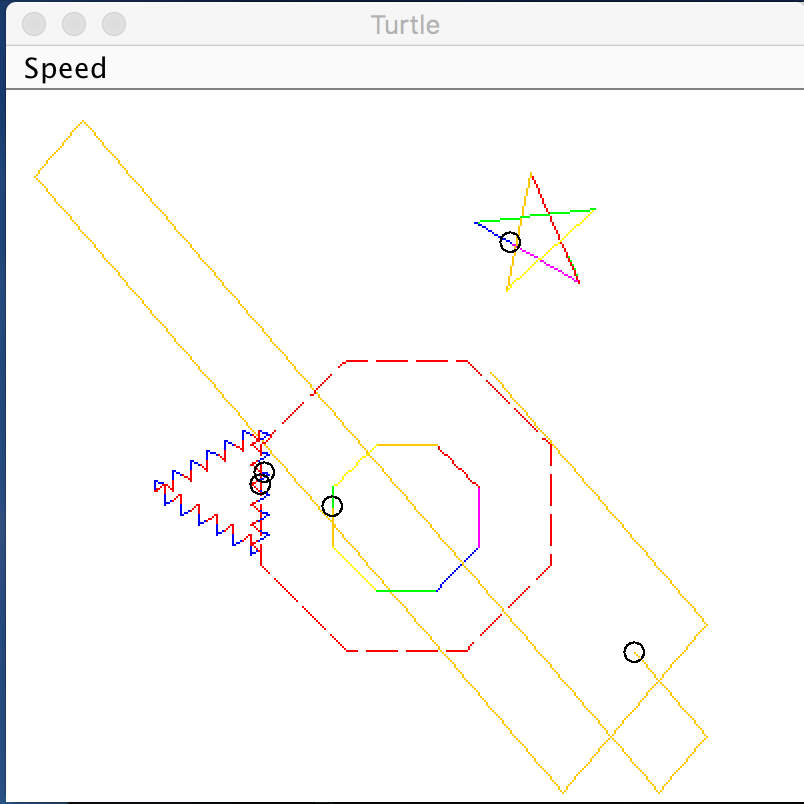
\includegraphics{ex3.png}
    \caption{問題3の実行結果}
    \label{emb}
  \end{center}
\end{figure}

\section{考察}
\subsection{負の長さを指定した三角形や初期座標が負の値をエラーにする}
負の値が入力されたり,引数を与えたりすると例外処理を行うようなプログラムを記述すれば良い.

\subsection{多相性とは?}
クラス型変数が派生関係にある様々なクラス型のインスタンスを参照できることを多相性と呼ぶ.
同じメッセージを送ったときに,メッセージを受け取ったインスタンスがそのクラスによって違う振る舞いをすることを示す.

\subsection{オブジェクト指向とは}
オブジェクト指向の主な要素として,「カプセル化」「継承」「多相性」がある.
これらを用いることでプログラムの簡略化・冗長を防ぐこと・可読性などができ,ソフトウェア開発・保守等の効率性・ 柔軟性の向上が期待できるという利点.

\subsection{作成をしたプログラム}
今回作成したプログラムは,「任意の多角形を作成するプログラム」・「goメソッドで虹色の点線を描く」・「任意の多角形を虹色の点線で描くプログラム」を作成した

\end{document}
